% !TeX root = ../main.tex

\xchapter{基于模拟器的瓶颈分析和设计空间探索}{Bottleneck Analysis and Design-Space Exploration based on the Simulator}

\xsection{问题定义与归因方法}{Problem Definition and Attribution Methodology}\label{sec:c4_method}

\xsubsection{问题定义与研究路线}{Problem Definition and Research Roadmap}\label{subsec:c4_problem}

第三章已经给出了模拟器在因果一致性、DRAM 闭环时序与真实负载总周期上的精度结论，使其可以作为对多核神经网络芯片进行系统级评估的可信工具。在此基础上，本章要回答的具体问题可分为两类。第一类是瓶颈识别与瓶颈消除：在真实 DNN 负载下，单核与多核场景的端到端时间究竟由计算、片上网络背压还是访存等待主导，瓶颈在硬件配置发生变化时是被消除还是被迁移。尤其是在多核映射与片外带宽提升之后，新的限速环节是否会出现在片上供数路径上。第二类是设计空间扩展上限：在确定一组合理的存储配置之后，多核神经网络芯片沿单核算力、核数与批量三个维度扩展时，吞吐能否随之线性增长，每个维度的扩展上限来自计算、互连还是存储侧。

围绕上述两类问题，本章组织两组前后衔接的实验。第一组以单核为起点，先在简化后端下完成 ResNet34 与 ResNet50 的端到端阶段占比分解，建立可解释的归因坐标系。再以同一坐标系把分析对象扩展至 4 核 ResNet50 的真实多核场景，沿先 DDR4、再升级到 HBM、最后加宽 SRAM 端口的递进路线进行三轮模拟，每一轮的硬件改动都由前一轮模拟暴露的瓶颈结论触发。第二组在第一组确定的最优存储配置之上，沿单核算力、核数与批量三个维度展开 12 组配置的扫描，定量给出各维度的扩展上限与设计启示。两组实验在归因口径上完全一致，由此保证它们的结论可以在同一框架下相互对照。

\xsubsection{阶段占比分解}{Phase-wise Time Decomposition}\label{subsec:c4_decomp}

为把端到端时间归因到具体的硬件资源，本文把每核每周期所处的状态划分为计算、片上网络背压与访存等待三类，并采用如下可复现的近似拆分：
\begin{equation}
  T_\text{COMPUTING} = \sum_c C^\text{comp}_c\label{eqn:c5:bottleneck_compute}
\end{equation}
\begin{equation}
  T_\text{NoC\_Stall} = \sum_c C^\text{nocstall}_c\label{eqn:c5:bottleneck_nocstall}
\end{equation}
\begin{equation}
  T_\text{Mem\_Stall} \approx \sum_c C^\text{wb}_c + \sum_c C^\text{load}_c - \sum_c C^\text{nocstall}_c\label{eqn:c5:bottleneck_memstall}
\end{equation}
式中：$T_\text{COMPUTING}$ 为端到端总计算时间，由各核 COMPUTING 阶段周期 $C^\text{comp}_c$ 求和得到。$T_\text{NoC\_Stall}$ 为端到端 NoC 背压时间，由各核因网络背压而停滞的周期 $C^\text{nocstall}_c$ 求和得到。$T_\text{Mem\_Stall}$ 为端到端访存相关等待时间，近似为各核 WRITEBACK 阶段周期 $C^\text{wb}_c$ 与 LOADING 阶段周期 $C^\text{load}_c$ 之和减去已计入的 NoC 背压。下标 $c$ 为核心索引。单核场景下无核间通信，故 $T_\text{NoC\_Stall}=0$，瓶颈主要体现在计算与访存（DRAM 读/写）的占比上。

\xsubsection{按核可视化与热点核定义}{Per-core Visualization and Hot-core Definition}\label{subsec:c4_percore}

阶段占比分解给出的是端到端的全局占比，而多核场景下不同核的负载与等待往往并不均衡，因此本文在此基础上进一步引入按核维度的可视化，作为对全局占比的空间补充。该可视化不引入新的模拟运行，而是直接利用模拟器为每核记录的状态时间线：在双核微基准上以各核各阶段占该核活跃时间的比例热力图呈现，在单核真实负载上以与分解口径一致的阶段占比堆叠条呈现。

热点核在本文中定义为：在给定维度（如总周期占比、计算周期占比、访存等待周期占比或 NoC 背压周期占比）上显著高于其他核心的核。模拟器在运行时可记录每个核心在每一模拟周期内所处的状态（加载、计算、写回或停滞），形成按核、按时间排列的状态时间线，据此可统计各核在各阶段的累计周期数，进而识别计算或等待时间最长的若干核心。

\xsection{性能瓶颈优化实验}{Performance Bottleneck Optimization Experiments}\label{sec:c4_bottleneck}

在前一章验证了模拟器的核间因果一致性、DRAM 闭环正确性与端到端总周期精度的基础上，本节围绕识别瓶颈、解释瓶颈与消除瓶颈这一主线，基于本文模拟器对神经网络芯片在真实 DNN 负载下的性能瓶颈展开系统性分析与逐级优化。

\xsubsection{单核性能瓶颈分析实验}{Single-core Performance Bottleneck Analysis Experiment}
\label{subsec:c4_singlecore}\label{subsec:c5_singlecore}

本小节选取 ResNet34 与 ResNet50 两类负载，以调度器生成 IR 驱动模拟，沿用前一节给出的阶段占比分解与按核可视化方法，实现对单核性能瓶颈的可解释归因。

\subsubsection{实验设置}

实验过程上，采用 Gemini-Compiler-IR 中 ResNet34 与 ResNet50 的调度结果（与前一章 ZeBu 对比实验同源）作为输入，在单核、简化后端配置下运行模拟器。模拟结束后，从输出的每核统计中读取每个核心在加载、计算、写回以及因网络背压而停滞的周期数，按式（\ref{eqn:c5:bottleneck_compute}）至式（\ref{eqn:c5:bottleneck_memstall}）汇总为总计算时间 $T_\text{COMPUTING}$、NoC 背压时间 $T_\text{NoC\_Stall}$ 与访存相关等待时间 $T_\text{Mem\_Stall}$，并计算三者占总执行时间的百分比。单核下无核间通信，NoC 背压恒为 0，瓶颈主要体现在计算与访存的占比上。表中给出批大小 1 的分解结果。

\subsubsection{实验结果}

实验结果方面，表\ref{tab:bottleneck}给出 ResNet34 与 ResNet50 在批大小 1、单核下的总周期及 $T_\text{COMPUTING}$、$T_{\mathrm{NoC}}$、$T_{\mathrm{Mem}}$ 的周期与占比，本实验中 $T_{\mathrm{NoC}}=0$。

\begin{table}[H]
  \centering
  \caption{真实负载端到端瓶颈分解表}
  \label{tab:bottleneck}
  \small
  \begin{tabular*}{\textwidth}{@{\extracolsep{\fill}}lrrcrccc}
    \toprule
    模型 & 总周期 & $T_\text{COMPUTING}$ & $T_{\mathrm{NoC}}$ & $T_{\mathrm{Mem}}$ & 计算\% & NoC\% & 访存\% \\
    \midrule
    ResNet34 & 1,890,695 & 1,530,664 & 0 & 359,888 & 81.0 & 0.0 & 19.0 \\
    ResNet50 & 2,432,592 & 1,863,694 & 0 & 568,717 & 76.6 & 0.0 & 23.4 \\
    \bottomrule
  \end{tabular*}
\end{table}

\begin{figure}[H]
  \centering
  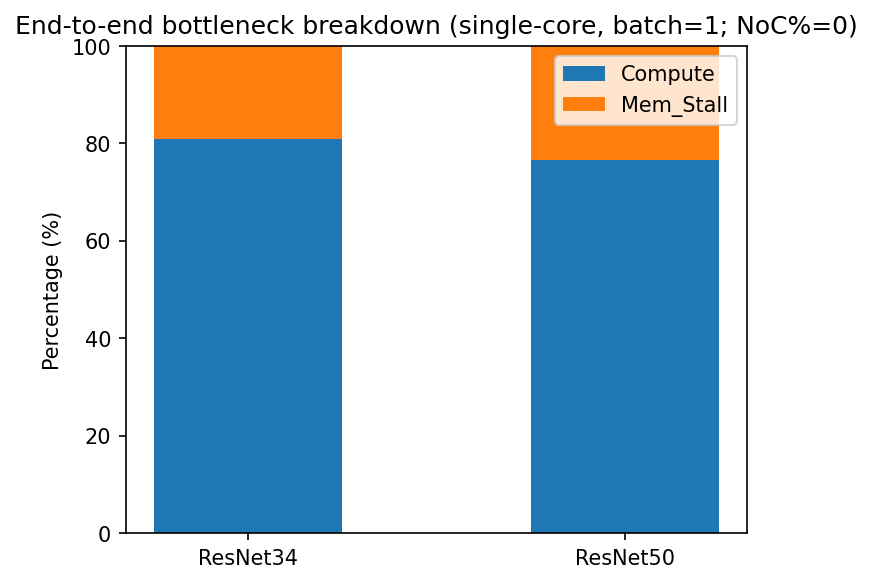
\includegraphics[width=0.65\linewidth]{Figures/c5_breakdown.png}
  \caption{端到端瓶颈占比图}
  \label{fig:c5_breakdown}
\end{figure}

\begin{figure}[H]
  \centering
  
\includegraphics[width=0.88\linewidth]{Figures/c5_522_hotspot_mb1.png}
  \caption{片上网络同步实验双核各阶段占该核活跃时间的比例热力图}
  \label{fig:c5_hot_cores}
\end{figure}

可视化数据来源与结果如下：（1）双核基准：复用前一章片上网络同步实验在简化后端下的双核点对点依赖负载状态轨迹，由各核工作负载的加载、计算、写回周期按核归一化，得到各阶段占该核活跃时间的比例，绘制热点热力图（图\,\ref{fig:c5_hot_cores}）。（2）单核真实负载（ResNet34/50）：直接复用上文批大小 1、单核的统计结果，将 $T_\text{COMPUTING}$ 与 $T_\text{Mem\_Stall}$ 占总时间的比例以堆叠条呈现，与表\ref{tab:bottleneck} 及图\,\ref{fig:c5_breakdown} 一致。

\subsubsection{实验分析}

对端到端结果（表\ref{tab:bottleneck}）的分析如下：（1）NoC 背压为 0。单核下无核间通信，$T_{\mathrm{NoC}}=0$，与预期一致。（2）计算为主导瓶颈。ResNet34 与 ResNet50 的计算占比分别为 81.0\% 与 76.6\%，说明在单核配置下端到端时间主要由计算阶段占据，与两类 CNN 的计算密度相符。（3）访存占比随模型加深而上升。ResNet50 的访存占比（23.4\%）高于 ResNet34（19.0\%），与 ResNet50 层数更多、中间激活与权重量更大、DRAM 读写的相对占比升高一致。多核映射下核间依赖与 NoC 竞争将引入非零 $T_\text{NoC\_Stall}$，届时可用同一分解框架区分计算与通信/访存瓶颈。

按核可视化方面，图\,\ref{fig:c5_hot_cores} 表明，在片上网络同步实验中 Core\,1 的加载阶段占该核活跃时间的比例显著高于 Core\,0，与 consumer 需同时等待 DRAM 与 Core\,0 数据的设定一致。计算阶段 Core\,0 占比更高，体现生产者核以计算为主、消费者核以等待与写回为主的分工。与前一章片上网络同步实验表\ref{tab:mb1} 及因果一致性结论一致，Core\,0 先完成加载与计算，Core\,1 在长时间加载后方进入计算与写回。图\,\ref{fig:c5_breakdown} 与表\ref{tab:bottleneck} 一致地表明，单核 ResNet 端到端时间仍以计算为主、访存相关等待次之，ResNet50 的访存占比高于 ResNet34，单核真实负载上的阶段占比条与上文宏观分解一致。

综上，单核场景下 ResNet34 / ResNet50 的端到端时间以计算为主导（占比约 77\%--81\%）、访存次之（19\%--23\%）、NoC 背压恒为 0，访存占比随模型加深而上升。按核可视化进一步揭示了生产者—消费者分工下的核间负载差异。本小节构建的分解口径 + 按核可视化框架既给出全局占比，也给出按核分布，将作为后续多核存储瓶颈定位与逐级优化实验的统一归因工具。

\xsubsection{多核存储瓶颈定位与逐级优化实验}{Multi-core Memory Bottleneck Identification and Iterative Optimization Experiment}
\label{subsec:c4_multicore}\label{subsec:c5_multicore}

前一小节在单核配置下建立了端到端瓶颈分解与按核可视化的归因框架。本小节将分析对象扩展到 4 核场景，使用高保真后端（BookSim2 + Ramulator2）运行真实 DNN 负载，沿DDR4 基线、HBM 升级、SRAM 端口加宽的递进路线进行三轮模拟。每一轮的硬件改动均由前一轮模拟暴露的瓶颈结论触发，最终在迭代中依次消除片外带宽与片上供数两类瓶颈。本小节后续所有图表均共享同一组实验设置：负载为 ResNet50，批大小为 1，4 核拓扑，采用高保真后端。三组 DRAM/SRAM 配置依次为 DDR4 单通道基线、HBM 四通道优化以及 HBM 四通道与 \SI{1024}{B/cycle} 宽 SRAM 端口的组合。后续 caption 中不再重复这些公共参数。

\subsubsection{实验设置}

本小节的实验设置围绕三个目标依次推进：先构造一个存储受限的多核基线配置，使 DRAM 带宽成为性能瓶颈，在甘特图上直观表现为加载阶段占据大部分时间。继而将 DRAM 技术从 DDR4 升级为 HBM（高带宽存储器），展示带宽升级对端到端性能的改善，以此验证模拟器能正确反映 DRAM 子系统差异。最后在 HBM 升级暴露出片上 SRAM 写端口瓶颈后，进一步加宽 SRAM 端口，观察三阶段是否趋于平衡。

在负载与 IR 生成方面，本节采用 ResNet50 网络，批大小为 1，通过 Gemini 编译器的 4 核映射模式生成调度 IR。IR 共含 288 个工作负载（每核 72 个），涉及约 \SI{90}{MB} 的 DRAM 读取与 288 次 DRAM 写回，涵盖了 ResNet50 全部卷积、池化与全连接层。

硬件配置上，两组配置共享相同的核心微架构（MAC 256、Vector 64、SRAM \SI{16}{MB}、核频 \SI{25}{MHz}）与 NoC 拓扑（4 核 Mesh，BookSim2 后端），差异仅在 DRAM 子系统：

\begin{table}[H]
  \centering
  \caption{多核瓶颈分析实验的两组 DRAM 配置表}
  \label{tab:c5_dram_configs}
  \small
  \begin{tabular*}{\textwidth}{@{\extracolsep{\fill}}ccc}
    \toprule
    参数 & DDR4 基线 & HBM 优化 \\
    \midrule
    DRAM 标准      & DDR4-2400R  & HBM-2Gbps \\
    通道数         & 1           & 4 \\
    Rank 数        & 1           & 1 \\
    峰值带宽       & \SI{19.2}{GB/s}  & \SI{128.0}{GB/s} \\
    等效带宽/核周期 & \SI{768}{B/cycle} & \SI{5120}{B/cycle} \\
    \bottomrule
  \end{tabular*}
\end{table}

DDR4 基线采用单通道以模拟带宽受限场景（峰值 \SI{19.2}{GB/s}），HBM 优化采用 4 通道 HBM（峰值 \SI{128.0}{GB/s}），峰值带宽提升约 6.7 倍。两组均使用 Ramulator2 后端，具备 DDR 行列时序、Bank 冲突与请求排队的全真建模。受行/Bank 冲突与 FR-FCFS 调度约束，实测有效带宽通常显著低于上述峰值，在 ResNet50 的 DRAM 访问模式下尤为明显，因此 DDR4 单通道仍会构成显著的访存瓶颈。

\subsubsection{第一轮：DDR4 基线模拟}

作为递进式优化的起点，第一轮模拟先在 DDR4 单通道配置下运行，目的是建立带宽受限的初始基线并据此定位首个性能瓶颈，为下一轮的硬件改动提供依据。表\ref{tab:c5_baseline_stats}给出 DDR4 基线配置下的模拟统计结果。

总周期为 238,803。各核加载阶段占活跃时间的 60\%--65\%，计算阶段仅 9\%--10\%，写回阶段约 26\%--28\%。LOADING\allowbreak /COMPUTING \allowbreak 总比值达 6.6，表明系统处于严重的存储受限状态。图\ref{fig:c5_hotspot_ddr4}以热力图形式展示了各核各阶段占活跃时间的比例，LOADING 列颜色最深，直观反映 DRAM 带宽瓶颈。

\begin{table}[H]
  \centering
  \caption{DDR4 基线模拟每核统计表}
  \label{tab:c5_baseline_stats}
  \small
  \begin{tabular*}{\textwidth}{@{\extracolsep{\fill}}crrrrc}
    \toprule
    核 & IDLE & LOADING & COMPUTING & WRITEBACK & Workloads \\
    \midrule
    0  & 0      & 140,680  & 22,352  & 64,537  & 72 \\
    1  & 0      & 153,077  & 22,352  & 58,929  & 72 \\
    2  & 0      & 144,515  & 22,352  & 66,362  & 72 \\
    3  & 0      & 153,799  & 22,352  & 62,381  & 72 \\
    \midrule
    总计 & --- & 592,071 & 89,408 & 252,209 & 288 \\
    \bottomrule
  \end{tabular*}
\end{table}

\begin{figure}[H]
  \centering
  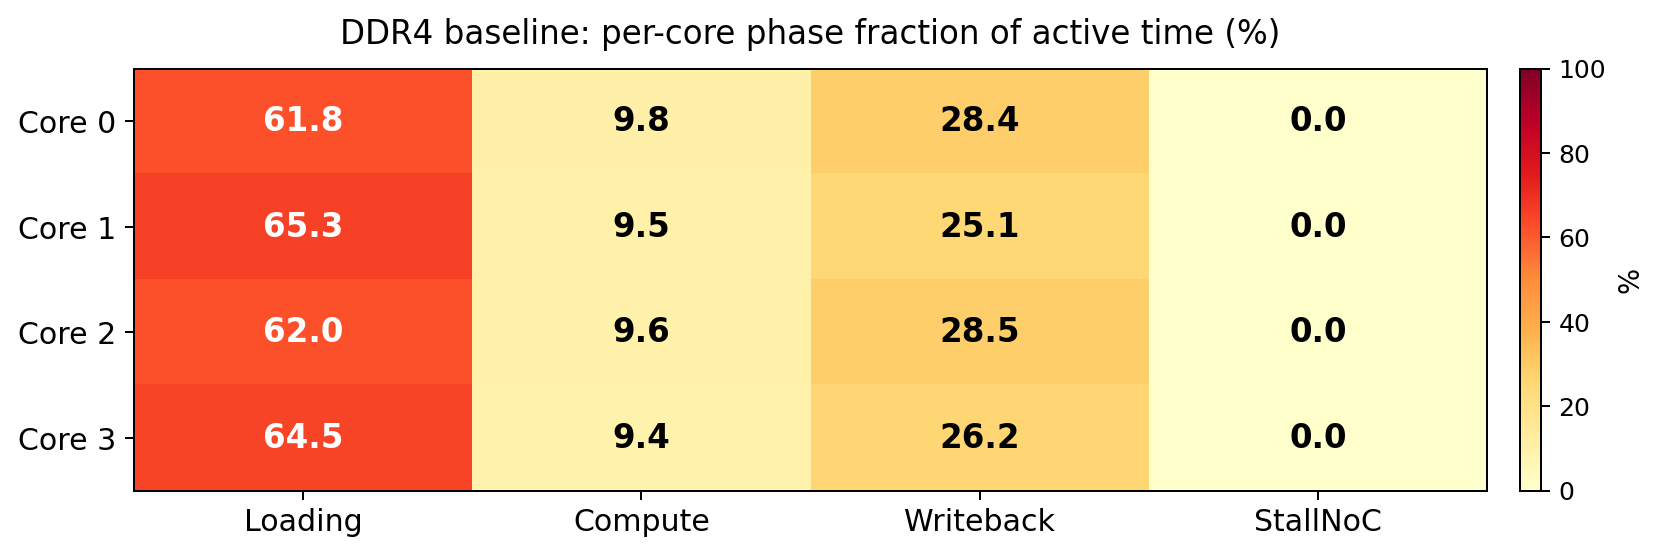
\includegraphics[width=0.88\linewidth]{Figures/c5_hotspot_ddr4_baseline.png}
  \caption{DDR4 基线各核阶段占比热力图}
  \label{fig:c5_hotspot_ddr4}
\end{figure}

图\ref{fig:c5_gantt_ddr4}给出 DDR4 基线的甘特图，实验条件为 4 核网格、ResNet50、批 1，颜色含义为橙色表示加载阶段（含 DRAM 读取与核间等待）、蓝色表示计算、红色表示写回。可见 4 核的加载段（橙色，含 DRAM 等待与核间等待子段）占据绝大部分时间线，计算段（蓝色）极为狭窄，直观展示了带宽瓶颈。

\begin{figure}[H]
  \centering
  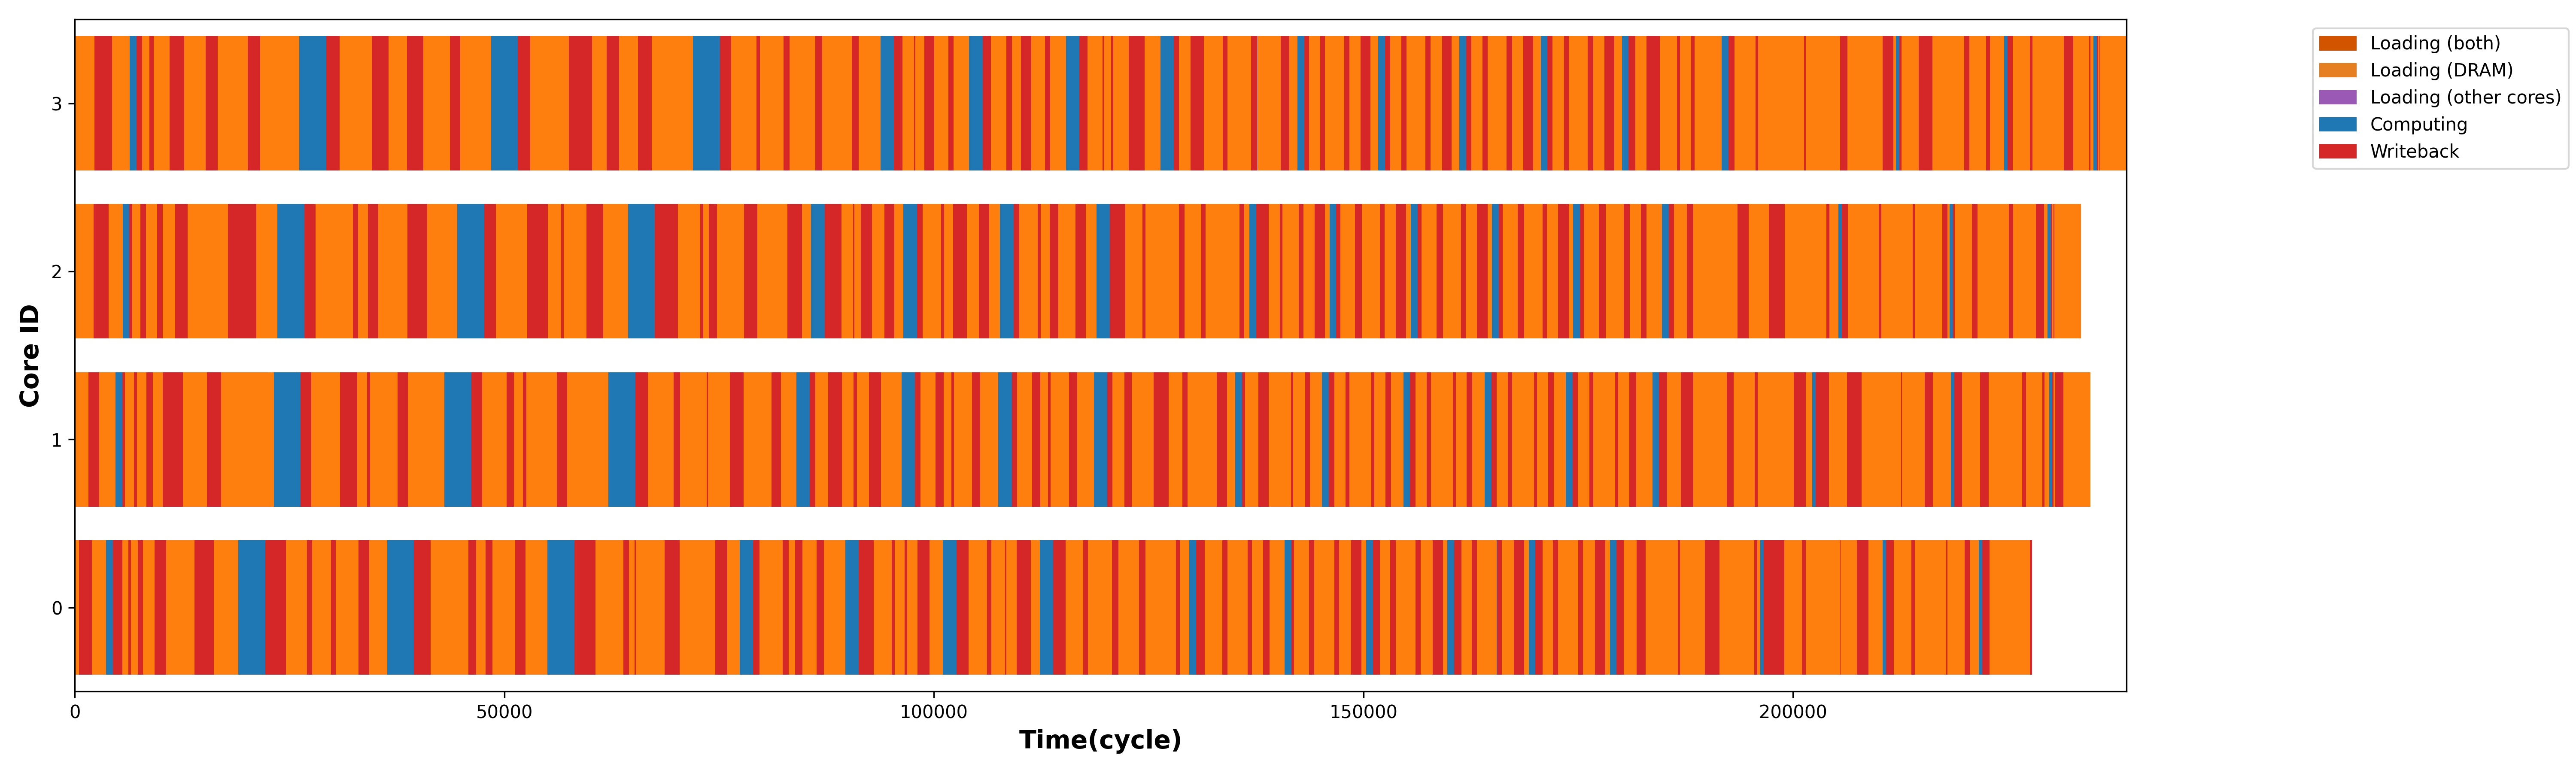
\includegraphics[width=\linewidth]{Figures/c5_gantt_ddr4_baseline.png}
  \caption{DDR4 基线甘特图}
  \label{fig:c5_gantt_ddr4}
\end{figure}

\subsubsection{第二轮：HBM 升级模拟}

第一轮模拟将瓶颈定位在 DDR4 单通道的 DRAM 带宽侧。第二轮即针对该瓶颈进行硬件改动，将 DRAM 从 DDR4 单通道替换为 HBM 四通道，使峰值带宽从 \SI{19.2}{GB/s} 提升至 \SI{128.0}{GB/s}，其余配置保持不变。在该配置下重新运行模拟以观察瓶颈是否消除或迁移，结果见表\ref{tab:c5_hbm_stats}。

\begin{table}[H]
  \centering
  \caption{HBM 优化模拟每核统计表}
  \label{tab:c5_hbm_stats}
  \small
  \begin{tabular*}{\textwidth}{@{\extracolsep{\fill}}crrrrc}
    \toprule
    核 & IDLE & LOADING & COMPUTING & WRITEBACK & Workloads \\
    \midrule
    0  & 0      & 84,488  & 22,352  & 18,092  & 72 \\
    1  & 0      & 102,664 & 22,352  & 18,713  & 72 \\
    2  & 0      & 85,616  & 22,352  & 18,093  & 72 \\
    3  & 0      & 97,415  & 22,352  & 18,533  & 72 \\
    \midrule
    总计 & --- & 370,183 & 89,408 & 73,431 & 288 \\
    \bottomrule
  \end{tabular*}
\end{table}

总周期降至 144,000。LOADING/COMPUTING 比值从 6.6 降至 4.1，WRITEBACK 总周期从 252,209 降至 73,431（降幅 70.9\%）。图\ref{fig:c5_hotspot_hbm}的热力图显示，LOADING 占比仍在 67\%--71\%（因 SRAM 端口瓶颈），但 WRITEBACK 从 25\%--28\% 降至 13\%--15\%，COMPUTING 从 9\%--10\% 升至 16\%--18\%。图\ref{fig:c5_gantt_hbm}为 HBM 优化甘特图，可见写回段（红色）显著收窄，加载段虽仍为主导但已明显缩短。

\begin{figure}[H]
  \centering
  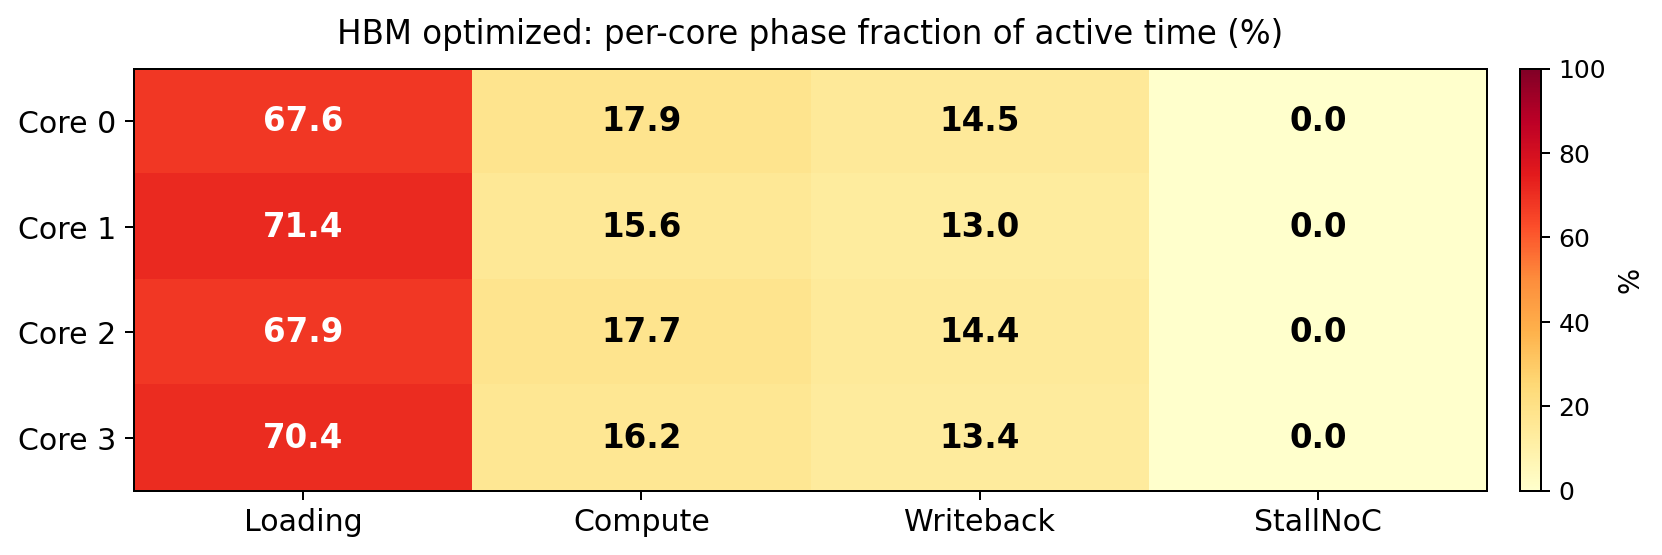
\includegraphics[width=\linewidth]{Figures/c5_hotspot_hbm_optimized.png}
  \caption{HBM 优化各核阶段占比热力图}
  \label{fig:c5_hotspot_hbm}
\end{figure}

\begin{figure}[H]
  \centering
  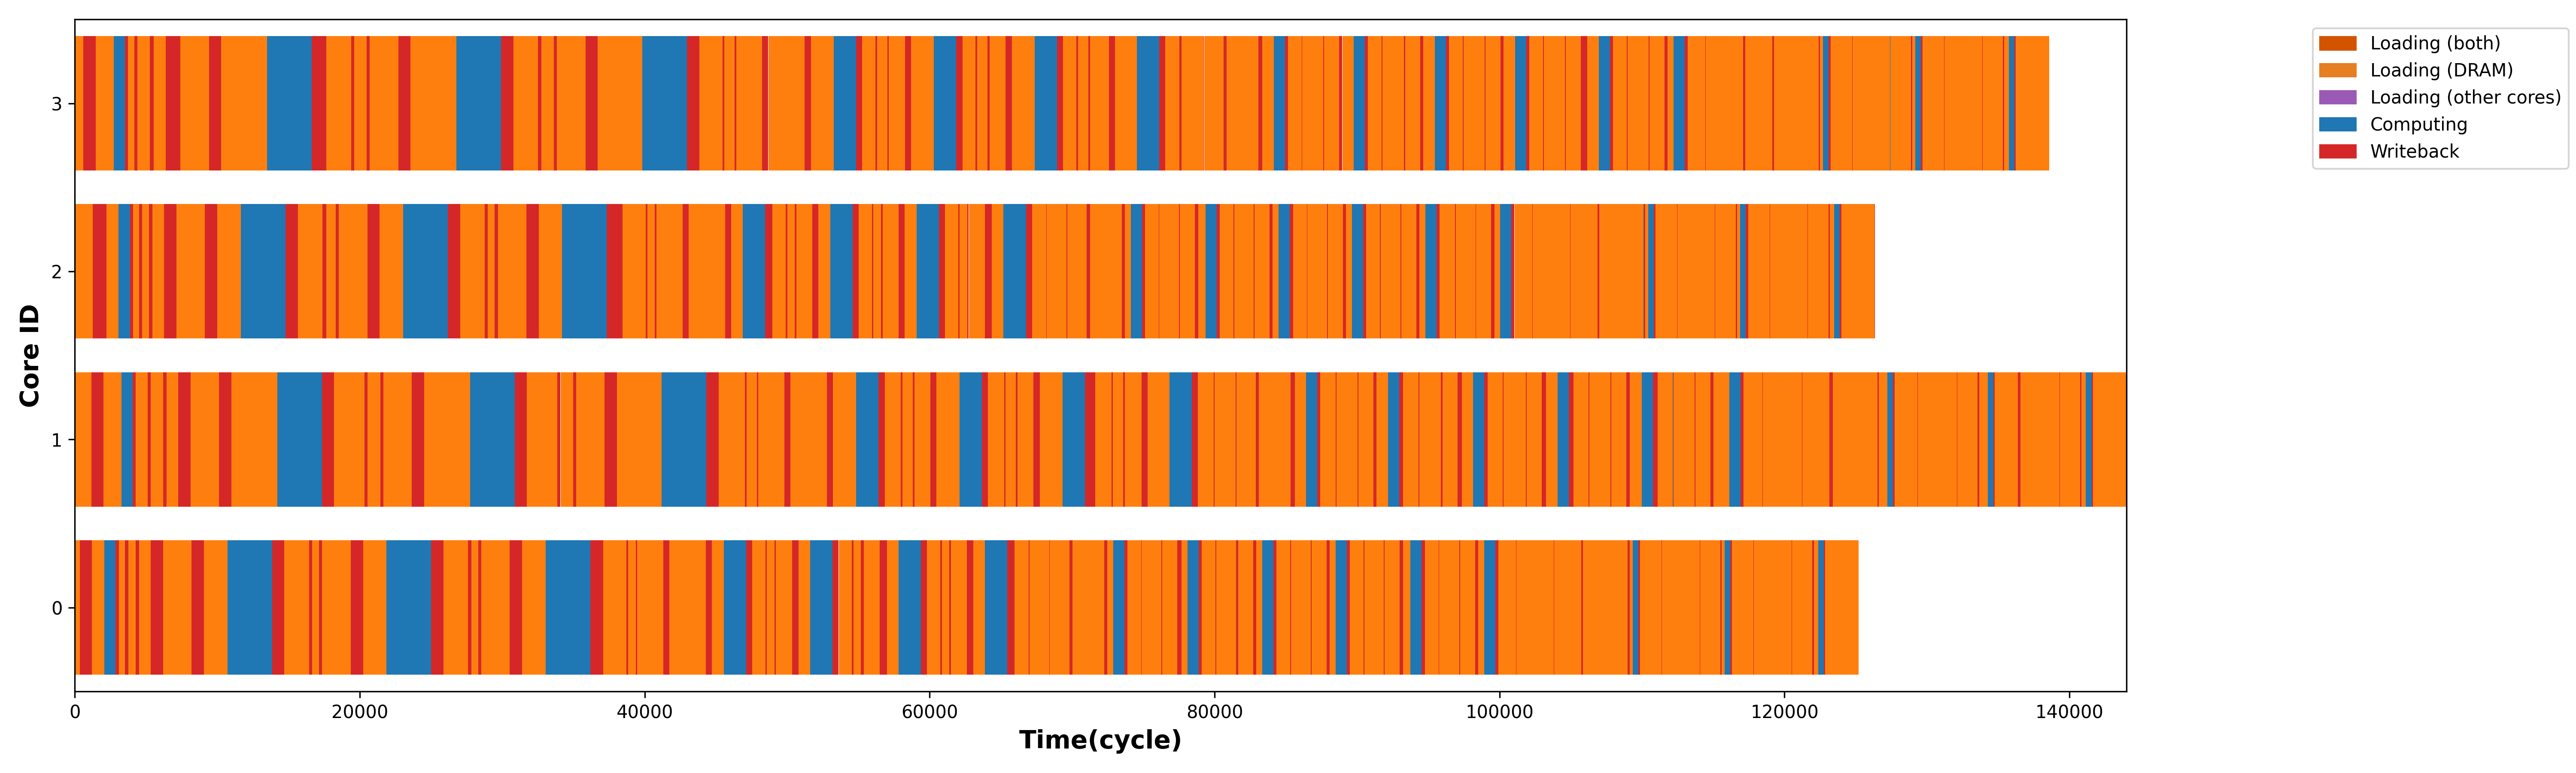
\includegraphics[width=\linewidth]{Figures/c5_gantt_hbm_optimized.png}
  \caption{HBM 优化甘特图}
  \label{fig:c5_gantt_hbm}
\end{figure}

对该轮模拟的残留瓶颈进行进一步分析可知，虽然 HBM 的峰值 DRAM 带宽达到 \SI{128}{GB/s}（\SI{5120}{B/cycle}），远超加载数据所需，但加载阶段仍占各核活跃时间的约 60\%。对 288 个工作负载的逐项分析表明：92\% 的工作负载的加载时间受 SRAM 写端口带宽限制（\SI{256}{B/cycle}）。具体而言，DRAM 数据到达核后必须按 SRAM 写带宽逐周期写入片上存储。当 DRAM 带宽远超 SRAM 写入速率时，后者成为新的瓶颈。

\subsubsection{第三轮：SRAM 端口加宽模拟}

第二轮模拟在 HBM 升级后将瓶颈从 DRAM 带宽迁移到了 SRAM 写端口。第三轮即针对这一新瓶颈再做硬件改动，将 SRAM 读写带宽从 \SI{256}{B/cycle} 提升至 \SI{1024}{B/cycle}，对应于在硬件设计上加宽 SRAM 读写端口或采用多 Bank 并行访问。除 SRAM 端口外，核微架构、NoC、DRAM 等其余参数保持不变。在新配置下重新运行模拟，以验证三阶段是否趋于平衡。

实验结果方面，表\ref{tab:c5_sram_stats}给出 HBM + SRAM \SI{1024}{B/cycle} 配置下的模拟统计。总周期降至 62,818，较 HBM（SRAM 256）再降 56.4\%，较 DDR4 基线降 73.7\%。LOADING\allowbreak /COMPUTING \allowbreak 比值从 4.1 降至 1.3，计算阶段占瓶颈核活跃时间的比例从 15.6\% 升至 35.7\%，系统从严重存储受限逐步趋向计算与存储的平衡。图\ref{fig:c5_hotspot_sram}的热力图显示，COMPUTING 占比升至 36\%--38\%，LOADING 降至 47\%--50\%，三阶段占比趋于均衡。图\ref{fig:c5_gantt_sram}的甘特图中，计算段（蓝色）面积明显增大，加载与写回段均大幅缩短。

\begin{figure}[H]
  \centering
  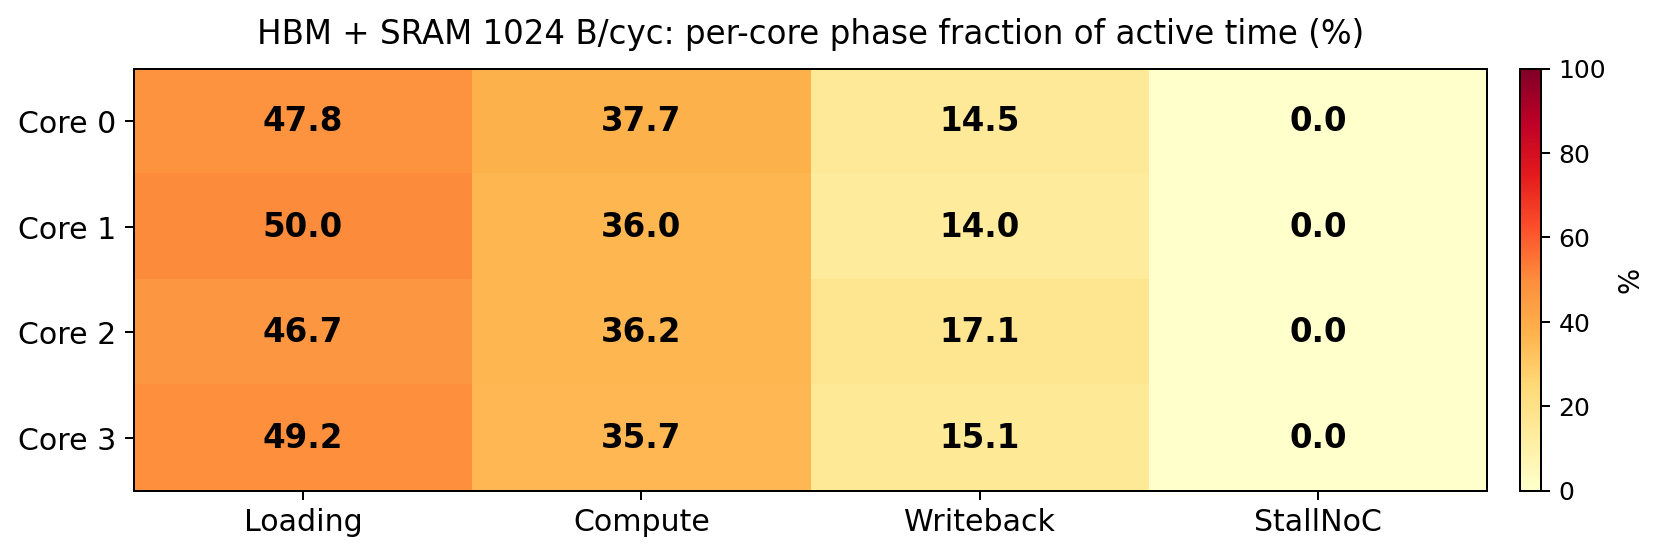
\includegraphics[width=0.8\linewidth]{Figures/c5_hotspot_hbm_sram1024.png}
  \caption{HBM + 宽 SRAM 各核阶段占比热力图}
  \label{fig:c5_hotspot_sram}
\end{figure}

\begin{figure}[H]
  \centering
  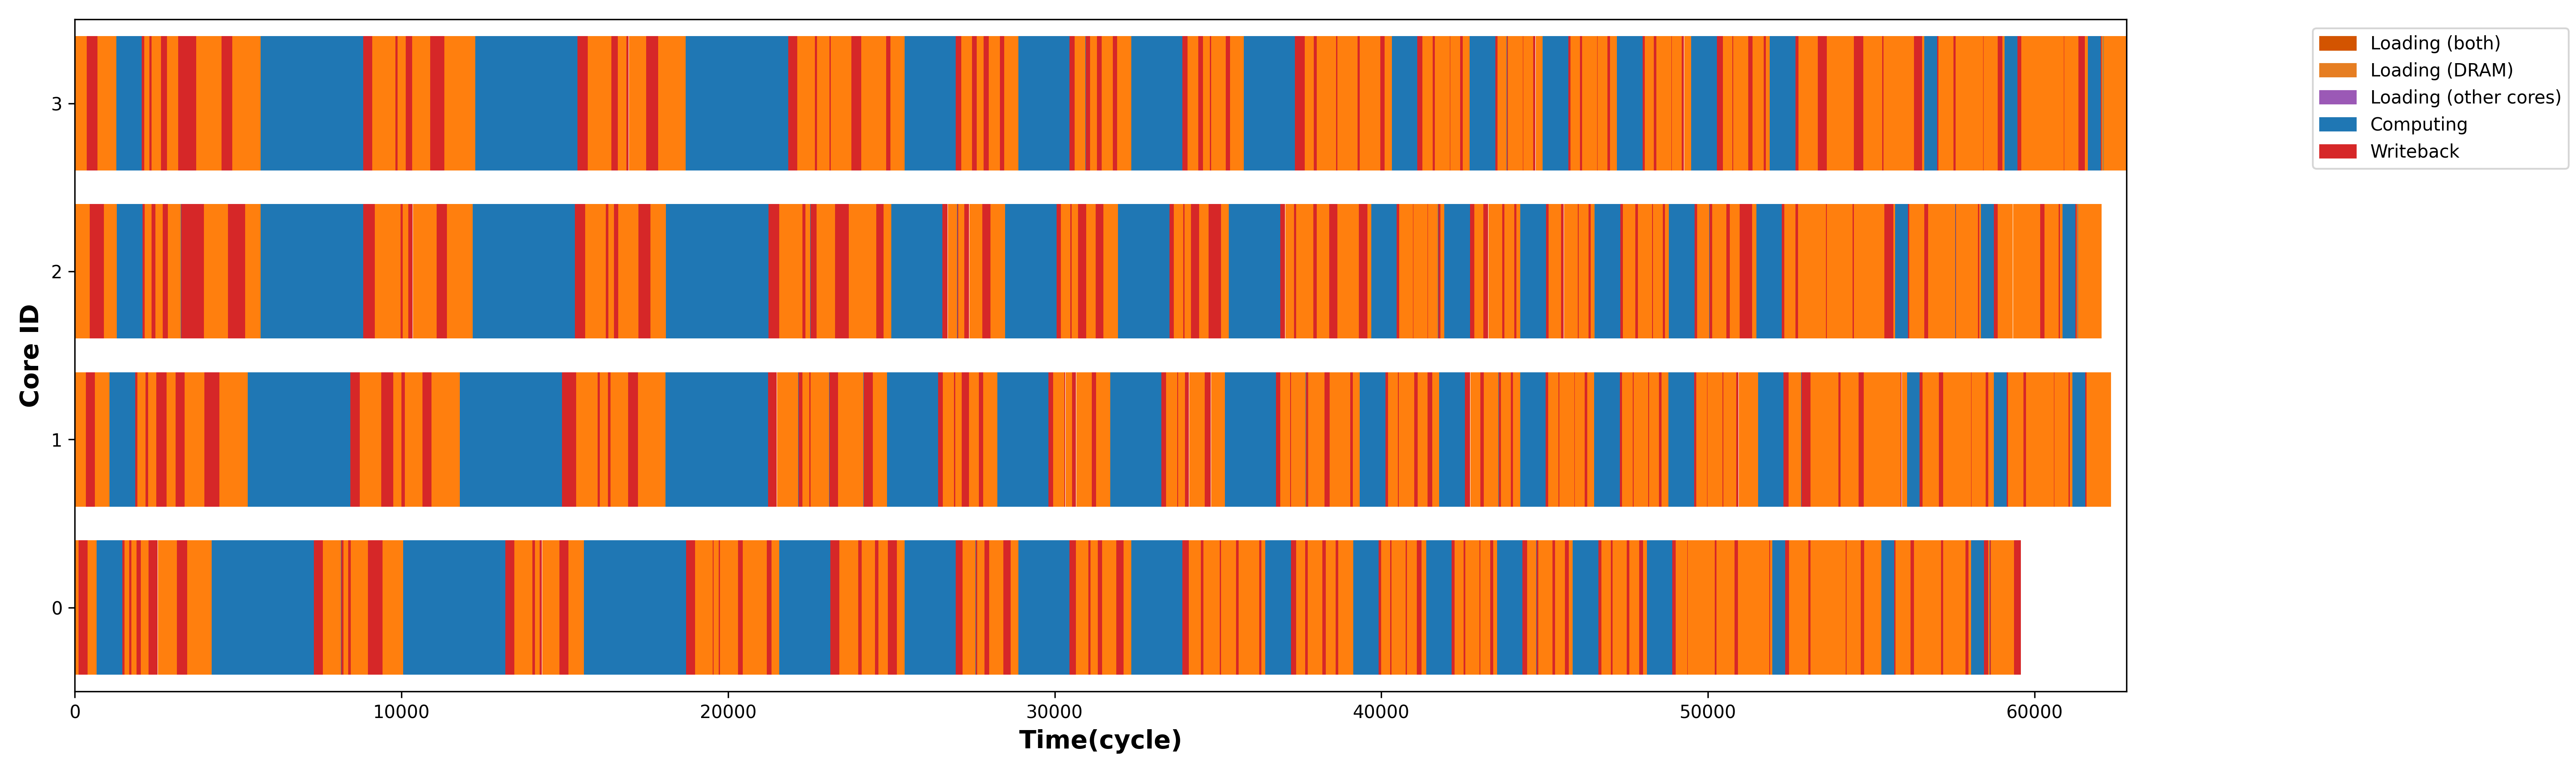
\includegraphics[width=0.8\linewidth]{Figures/c5_gantt_hbm_sram1024.png}
  \caption{HBM + 宽 SRAM 甘特图}
  \label{fig:c5_gantt_sram}
\end{figure}

\begin{table}[H]
  \centering
  \caption{HBM + 宽 SRAM 模拟每核统计表}
  \label{tab:c5_sram_stats}
  \small
  \begin{tabular*}{\textwidth}{@{\extracolsep{\fill}}crrrrc}
    \toprule
    核 & IDLE & LOADING & COMPUTING & WRITEBACK & Workloads \\
    \midrule
    0  & 0      & 28,374  & 22,352  & 8,589   & 72 \\
    1  & 0      & 31,058  & 22,352  & 8,668   & 72 \\
    2  & 0      & 28,853  & 22,352  & 10,588  & 72 \\
    3  & 0      & 30,766  & 22,352  & 9,429   & 72 \\
    \midrule
    总计 & --- & 119,051 & 89,408 & 37,274 & 288 \\
    \bottomrule
  \end{tabular*}
\end{table}

\subsubsection{三轮综合对比}

表\ref{tab:c5_comparison}汇总三组配置的关键指标，展示了优化路径的完整效果。

\begin{table}[H]
  \centering
  \caption{三组配置模拟结果对比表}
  \label{tab:c5_comparison}
  \small
  \begin{tabular*}{\textwidth}{@{\extracolsep{\fill}}lrrrc}
    \toprule
    指标 & DDR4 基线 & HBM 优化 & HBM+宽SRAM & 总改善 \\
    \midrule
    总周期            & 238,803   & 144,000  & 62,818   & $-$73.7\% \\
    相对DDR4加速比    & 1.00$\times$ & 1.66$\times$ & 3.80$\times$ & --- \\
    LOADING 总周期    & 592,071   & 370,183  & 119,051  & $-$79.9\% \\
    WRITEBACK 总周期  & 252,209   & 73,431   & 37,274   & $-$85.2\% \\
    COMPUTING 总周期  & 89,408    & 89,408   & 89,408   & 0\% \\
    LOADING/COMPUTING & 6.62       & 4.14      & 1.33      & --- \\
    瓶颈核计算占比    & 9.4\%      & 15.6\%    & 35.7\%    & --- \\
    DRAM 峰值带宽     & \SI{19.2}{GB/s} & \SI{128}{GB/s} & \SI{128}{GB/s} & --- \\
    SRAM 写带宽       & \SI{256}{B/cy}  & \SI{256}{B/cy} & \SI{1024}{B/cy} & --- \\
    \bottomrule
  \end{tabular*}
\end{table}

综上，沿DDR4 基线、HBM 升级、SRAM 端口加宽三轮递进，瓶颈先后从 DRAM 读写带宽迁移至片上 SRAM 写端口，再迁移至计算单元。总周期由 238,803 降至 62,818，相对基线达到 3.80 倍加速。LOADING/COMPUTING 比由 6.6 降至 1.3，而计算周期始终保持 22,352 时钟周期不变。这一逐级暴露新瓶颈、针对性优化、再次模拟的迭代过程揭示了高带宽外部存储下片上带宽墙现象的存在，也验证了模拟器在多核存储子系统设计空间探索中的实用价值。

\xsubsection{实验结论}{Experimental Conclusions}\label{subsec:c4_bot_conclusion}
\label{subsec:c5_bottleneck_overall}

综合前两小节的单核与多核实验，可以从归因方法、瓶颈现象与设计启示三个角度给出整体结论。

本节所构建的归因框架由分解口径与按核可视化两部分组成，在单核与多核两种规模下保持一致的口径。该框架将端到端时间严格拆分为计算、片上网络背压与访存等待三类周期，并同时支持全局占比汇总与按核空间分布展示。在应用层面，该框架既用于解释单核 ResNet 端到端时间的构成，也用作多核三轮递进模拟的判据，依据前一轮瓶颈结论决定下一轮硬件改动。这表明该框架具备跨规模、跨配置的通用归因能力，可作为后续设计空间探索的标准分析工具。

进一步对比单核与多核场景，可以发现瓶颈的相对地位差异显著。单核 ResNet34/50 上计算占比约 77\%--81\%，访存占比约 19\%--23\%，NoC 背压恒为 0。即使模型加深至 ResNet50，访存占比的上升也未改变计算主导的总体格局。一旦扩展到 4 核、ResNet50、DDR4 单通道的多核存储受限场景，访存等待则跃升为主导阶段，LOADING\allowbreak /COMPUTING \allowbreak 比可达 6.6。仅靠升级 DRAM（由 DDR4 升级到 HBM）无法消除该瓶颈，必须配合加宽 SRAM 端口，才能将该比值压回 1.3 量级。这表明从单核到多核的扩展并非简单的算力线性叠加，而会触发外部带宽与片上供数路径的连锁瓶颈，单一维度的硬件升级往往只是完成瓶颈迁移而非瓶颈消除。

由此可对未来神经网络芯片在算力与存储平衡上的设计提炼三点参考。其一，片外带宽、片上端口与计算阵列应作为整体协同的三层资源进行联合优化。单独提升任一层都可能因相邻层成为新瓶颈而损失收益，多核三轮迭代中 HBM 升级后 SRAM 写端口反成限速环节即为典型案例。其二，访存与计算的相对占比是判断系统是否处于计算受限、带宽受限或片上供数受限状态的可解释指标。建议在芯片早期架构探索中即以该指标作为权衡片上 SRAM 容量、端口宽度与外部 DRAM 配置的依据。其三，本文模拟器在迭代式硬件改动中能够保持各子系统贡献的可分离性，例如多核三轮迭代中各核计算时长恒为 22,352 时钟周期。这一性质使其能够准确反映各类硬件改动各自带来的收益，为多核神经网络芯片的设计决策提供定量证据。上述结论将作为后续多核吞吐量设计空间探索实验中各项参数选择（如 HBM 四通道与 \SI{1024}{B/cycle} SRAM 端口的组合）的依据。

\xsection{多核吞吐量设计空间探索实验}{Design-Space Exploration Experiment for Multi-core Throughput}\label{sec:c4_dse}
\label{sec:c5_dse}

在实际推理部署中，吞吐量受单核算力、核数规模、片上存储与 die 面积等多因素共同约束。本节沿单核算力（MAC 规模）、核数扩展与批量三个维度展开设计空间探索。所有实验均采用 ResNet50 网络、HBM 四通道 DRAM 与 \SI{1024}{B/cycle} SRAM 带宽（即前述多核三轮迭代确定的最优存储配置），并使用高保真后端（BookSim2 + Ramulator2）。后续 caption 中不再重复这些公共参数，仅在正文中说明每组实验所变动的维度与取值。

\xsubsection{单核算力扩展实验}{Single-core MAC Scaling Experiment}

在 4 核配置下，将单核乘法累加单元数从 256 扫描至 512 和 1024，对批量为 1 和批量为 4 各运行一组模拟。

表\ref{tab:c5_mac_sweep}给出 MAC 扫描结果。对实验结果的分析如下：三种 MAC 规模下的总周期几乎无差异（批量为 1 时均约 62,778，批量为 4 时均约 258,000），且 COMPUTING 总周期完全一致。这一看似反直觉的结果源于当前负载的特征：Gemini 编译器生成的 IR 中，288 个工作负载（批量为 1 时）有 75\% 的工作负载计算量极小（compute\_cycles $\leq$ 1），真正有显著计算的仅为 residual 层。即使将 MAC 翻四倍，瓶颈核的活跃时间仍由 LOADING 主导（L/C $\approx$ 1.33），计算缩减对总周期的贡献被淹没。结论：在当前存储配置下，系统处于存储受限状态，单纯提升单核算力无法提高吞吐量。

\begin{table}[H]
  \centering
  \caption{MAC 规模扫描表}
  \label{tab:c5_mac_sweep}
  \small
  \begin{tabular*}{\textwidth}{@{\extracolsep{\fill}}ccrrrrc}
    \toprule
    MAC & 批量 & 总周期 & LOADING & COMPUTING & WRITEBACK & 计算占比 \\
    \midrule
    256  & 1 & 62,775  & 119,210 & 89,408  & 36,944  & 35.8\% \\
    512  & 1 & 62,778  & 119,220 & 89,408  & 36,946  & 35.8\% \\
    1024 & 1 & 62,776  & 119,223 & 89,408  & 36,935  & 35.8\% \\
    \midrule
    256  & 4 & 258,289 & 508,269 & 357,632 & 153,289 & 34.8\% \\
    512  & 4 & 258,289 & 508,269 & 357,632 & 153,289 & 34.8\% \\
    1024 & 4 & 257,969 & 510,067 & 357,632 & 153,290 & 34.8\% \\
    \bottomrule
  \end{tabular*}
\end{table}

\xsubsection{核数扩展实验}{Core-count Scaling Experiment}

固定单核乘加器单元数量为 512，将核数从 4 核扩展至 16 核与 64 核。每种核数的 IR 由 Gemini 编译器针对对应拓扑重新生成。

实验结果方面，表\ref{tab:c5_core_sweep}给出核数扩展结果。对实验结果的分析如下：（1）核数由 4 扩展到 16：总周期几乎不降。批量为 1 时从 62,781 降至 60,839（仅 $-$3.1\%），批量为 4 时反而从 257,827 升至 296,297（$+$14.9\%）。原因在于：核数增加后工作负载被分散到更多核（从 288 增至 1136），但 16 核共享同一 DRAM 子系统导致读写竞争加剧，LOADING 与 WRITEBACK 剧增。L/C 从 1.33 升至 5.61（批量为 1 时）和从 1.42 升至 6.95（批量为 4 时），系统从接近均衡退回到严重存储受限。（2）64 核死锁。64 核配置下模拟无法完成：99.3\% 的工作负载完成后，剩余 30 个工作负载的 15 个核陷入互等状态。这是因为 ResNet50 的层级结构（约 72 个 unique 层）无法均匀分布到 64 核，Gemini 编译器生成的 IR 中大量核的工作负载极少，导致复杂的依赖链形成环路。结论：核数不宜超过负载的并行度上限。

\begin{table}[H]
  \centering
  \caption{核数扩展实验结果表}
  \label{tab:c5_core_sweep}
  \small
  \begin{tabular*}{\textwidth}{@{\extracolsep{\fill}}lcrrrrc}
    \toprule
    核数 & 批量 & 总周期 & L/C & 计算占比 & Workloads & 状态 \\
    \midrule
    4 & 1 & 62,781   & 1.33  & 35.8\% &  288 & 完成 \\
    16 & 1 & 60,839   & 5.61  & 9.2\%  & 1136 & 完成 \\
    64 & 1 & ---       & ---   & ---    & 4544 & 死锁 \\
    \midrule
    4 & 4 & 257,827  & 1.42  & 34.8\% & 1152 & 完成 \\
    16 & 4 & 296,297  & 6.95  & 7.6\%  & 4544 & 完成 \\
    \bottomrule
  \end{tabular*}
\end{table}

图\ref{fig:c5_hotspot_4x4_b1} 以热力图形式展示各核阶段占活跃时间的比例：全部核心的 LOADING 占比在 50\%--55\%，WRITEBACK 在 36\%--41\%，COMPUTING 仅约 9.3\%--9.5\%。该比例与多核三轮迭代中 DDR4 基线（4 核）的 9\%--10\% 接近，表明核数扩大 4 倍后系统从接近均衡退回到严重存储受限。图\ref{fig:c5_dse_4x4_b1} 给出对应的 16 核端到端甘特图，其中 LOADING 与 WRITEBACK 段占据绝大部分时间线，DRAM 争用严重。

\begin{figure}[H]
  \centering
  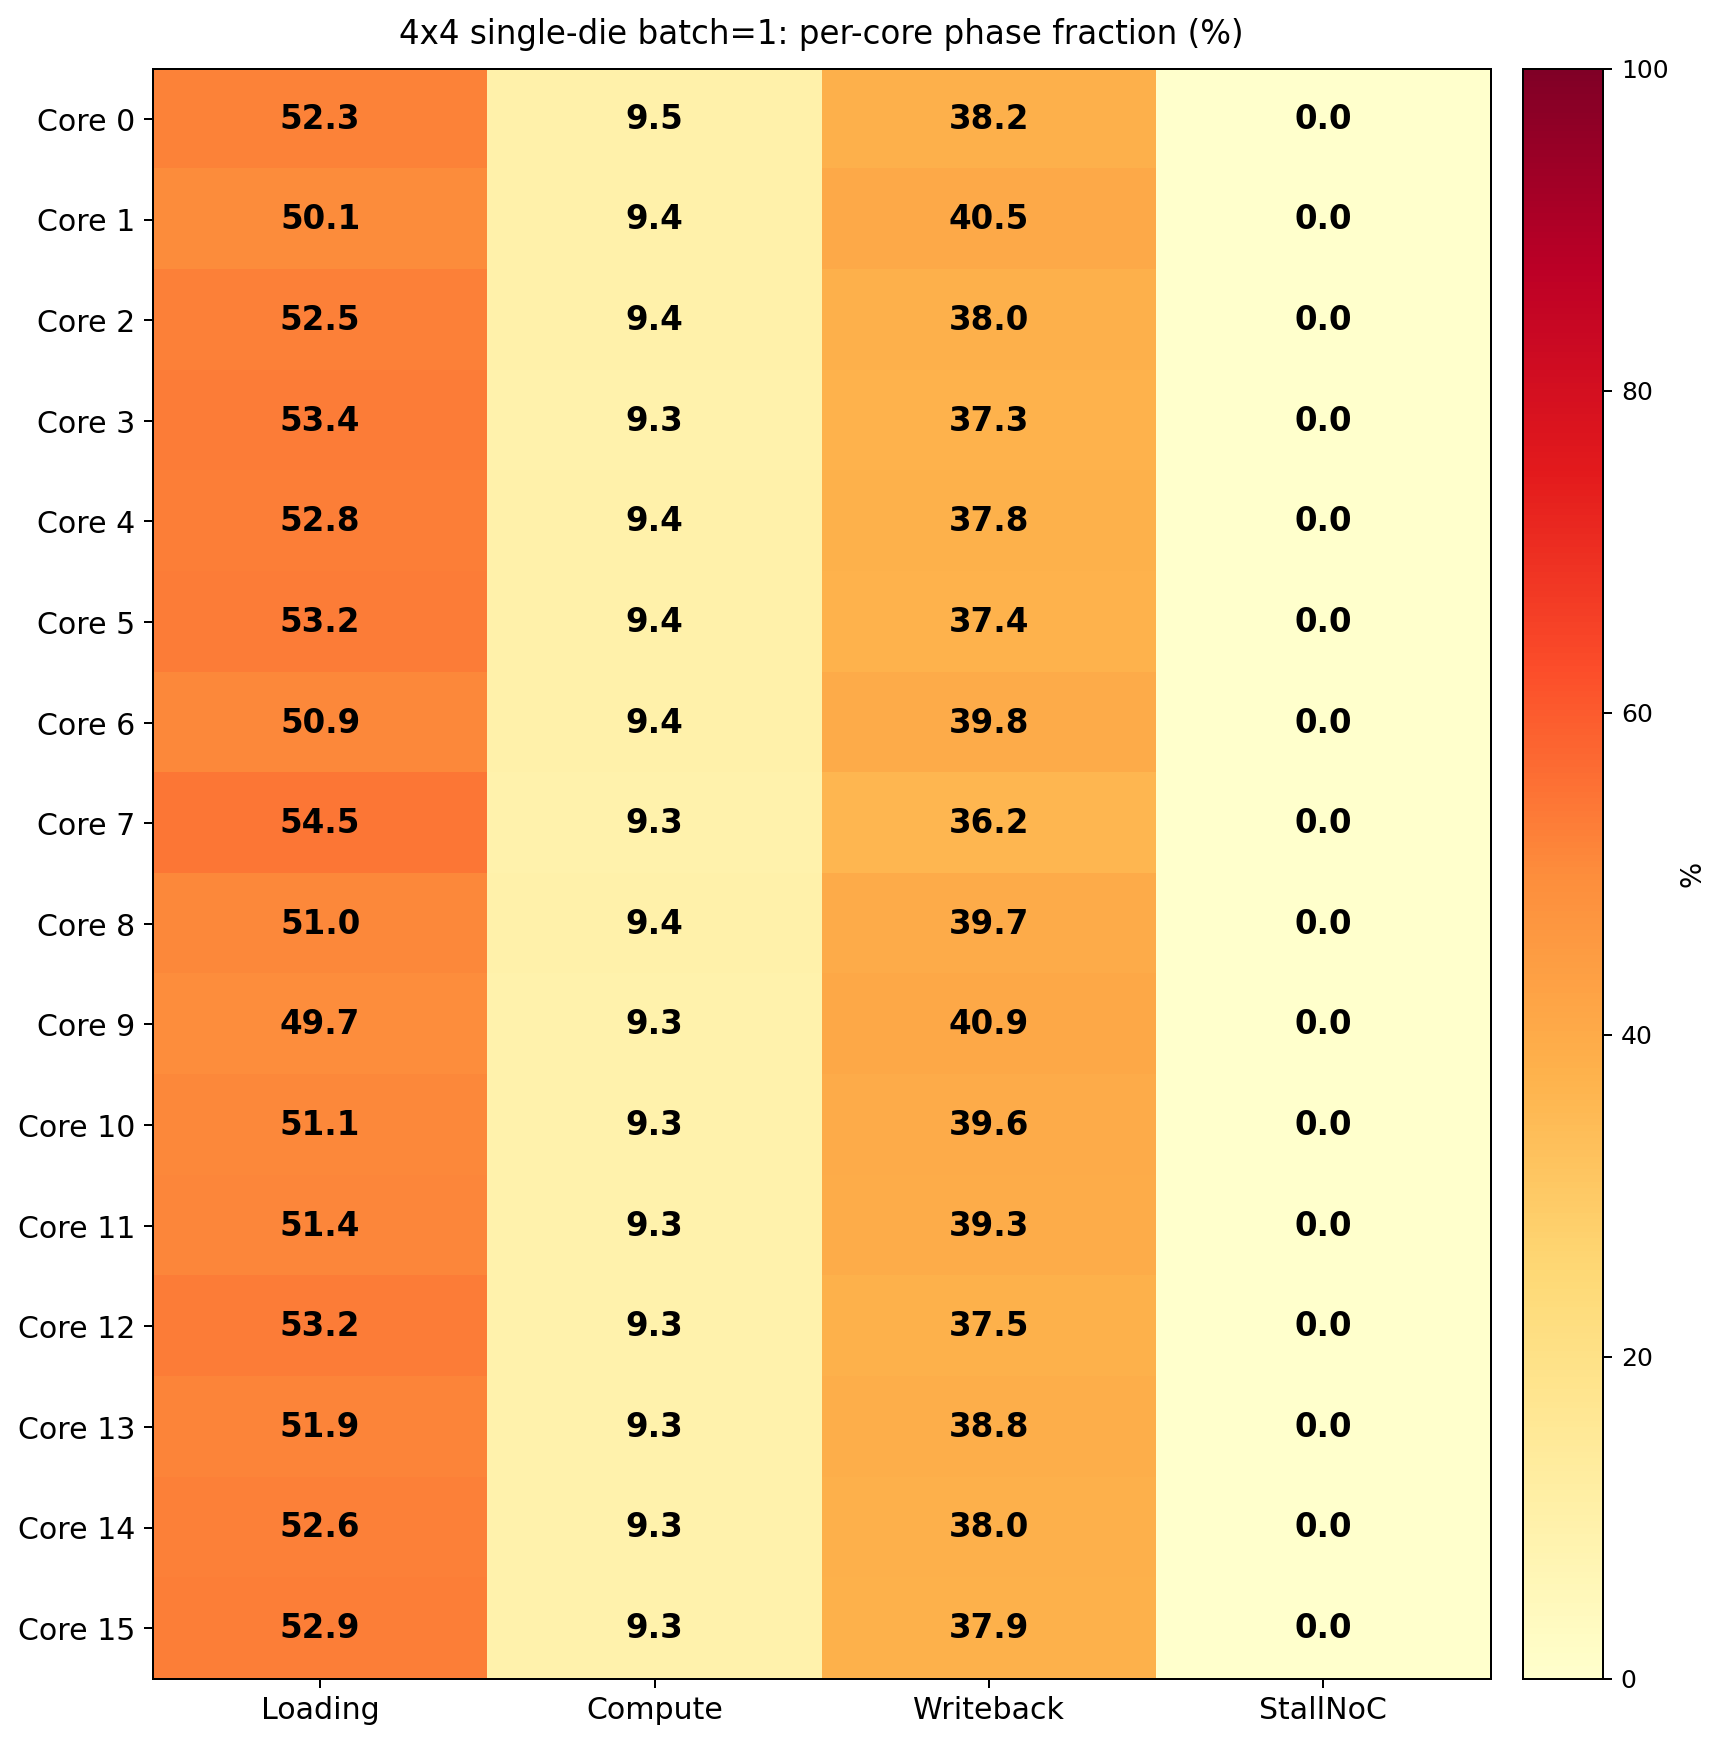
\includegraphics[width=0.8\linewidth]{Figures/c5_hotspot_4x4_b1.png}
  \caption{16 核各阶段占比热力图}
  \label{fig:c5_hotspot_4x4_b1}
\end{figure}

\begin{figure}[H]
  \centering
  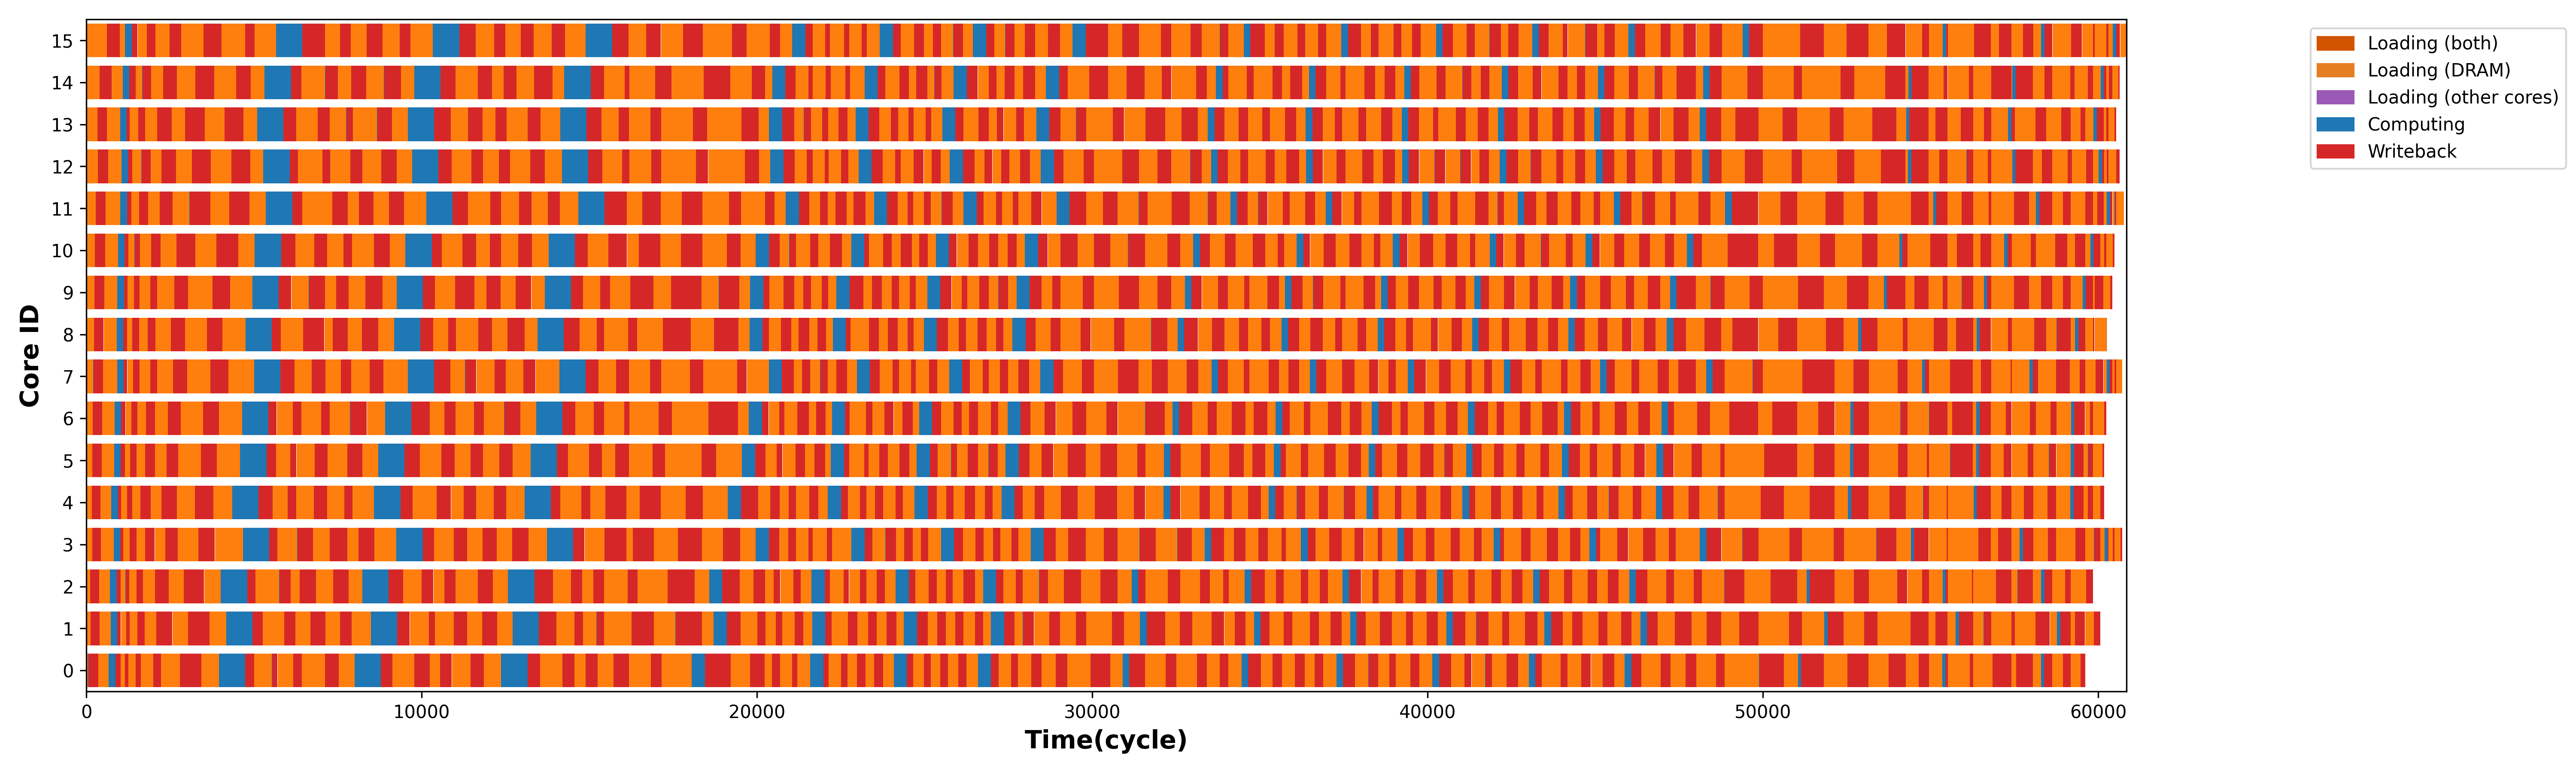
\includegraphics[width=\linewidth]{Figures/c5_dse_4x4_b1.png}
  \caption{16 核甘特图}
  \label{fig:c5_dse_4x4_b1}
\end{figure}

\xsubsection{批量扩展实验}{Batch Scaling Experiment}

在推理部署中，增大批量可以提高数据复用率与吞吐量。表\ref{tab:c5_batch}对比批量为 1 与批量为 4 在不同核数配置下的吞吐量。吞吐量定义为：
\begin{equation}
  \text{Throughput} = \frac{\text{Batch}}{\text{Total\_cycles}}\label{eqn:c5:throughput}
\end{equation}
式中：$\text{Throughput}$ 为单位周期完成的推理数。$\text{Batch}$ 为一次推理处理的样本数。$\text{Total\_cycles}$ 为完成该 Batch 推理所用的总仿真周期数。

对实验结果的分析如下：批量从 1 增至 4 时，总周期增长约 4.1 倍（4 核）到 4.9 倍（16 核），均超过批量本身的 4 倍，导致吞吐量反而略降。批量扩展效率（= 批量为 4 时吞吐量 / 批量为 1 时吞吐量 / 4）仅约 24\%。这是因为在当前存储受限配置下，增大批量线性增加了 DRAM 读写数据量，但 DRAM 带宽并未同步扩展，导致存储争用超线性增长。

\begin{table}[H]
  \centering
  \caption{批量扩展效率表}
  \label{tab:c5_batch}
  \small
  \begin{tabular*}{\textwidth}{@{\extracolsep{\fill}}lcrrrc}
    \toprule
    核数 & 批量 & 总周期 & 吞吐量（$\times 10^{-5}$/cyc） & 相对批量为 1 加速 & 效率 \\
    \midrule
    4 & 1 & 62,781  & 1.593 & ---     & --- \\
    4 & 4 & 257,827 & 1.551 & 0.97$\times$ & 24.3\% \\
    \midrule
    16 & 1 & 60,839  & 1.644 & ---     & --- \\
    16 & 4 & 296,297 & 1.350 & 0.82$\times$ & 20.5\% \\
    \bottomrule
  \end{tabular*}
\end{table}

\xsubsection{实验结论}{Experimental Conclusions}\label{subsec:c4_dse_conclusion}

多核吞吐量设计空间探索实验的 12 组实验对比分析结论如下：（1）存储受限状态下，提升算力无效。当 LOADING/COMPUTING $>$ 1 时，系统为存储受限，增加 MAC 单元对吞吐量无贡献。设计者应优先解决 DRAM 带宽或 SRAM 端口带宽瓶颈，再考虑计算资源投入。（2）核数扩展存在明确上限。核数由 4 扩展到 16 时，在批量为 1 时仅提升 3\%，在批量为 4 时反而退步 15\%，64 核 直接死锁。核数必须与负载的并行度匹配：ResNet50 的有效并行度约 4--16 核，超过此范围后 DRAM 争用与调度依赖冲突主导性能。（3）批量扩展效率受限于存储带宽。批量为 4 相对批量为 1 的吞吐量效率仅约 24\%，说明在存储受限系统中批量扩展的收益远不及理想的线性关系，提升 DRAM 通道数或采用更高带宽的 HBM2E/HBM3 可望改善批量扩展效率。（4）模拟器对神经网络芯片设计的价值。本节实验覆盖了 12 种配置组合，每次模拟耗时 3--60 分钟，这一效率使得在流片前对核数、算力、存储带宽等关键参数进行快速定界成为可能。


\xsection{本章小结}{Chapter Summary}\label{sec:c4_summary}

本章基于前一章的模拟平台，沿着识别瓶颈、消除瓶颈与探索设计空间这条主线开展了两组前后衔接的实证研究。

在归因方法上，本章建立了一套阶段占比分解与按核可视化结合的统一框架。该框架把端到端时间拆分为计算、片上网络背压与访存等待三类周期，并通过热力图呈现各核在各阶段的时间分布。

在瓶颈分析上，本章先在单核配置下完成 ResNet34 与 ResNet50 的端到端阶段分解，再在 4 核配置下进行三轮递进的模拟。三轮模拟先以 DDR4 为基线，再升级到 HBM，最后加宽 SRAM 端口。每一轮的硬件改动都由前一轮模拟暴露的瓶颈结论触发，从而依次消除片外带宽与片上供数两类瓶颈。

在设计空间探索上，本章在前一阶段确定的最优存储配置之上，沿单核算力、核数与批量三个维度扫描了 12 组配置，并据此得到三条结论。其一，在存储受限的情形下，提升 MAC 规模并不能带来线性的收益。其二，核数扩展存在明确的并行度上限。其三，批量扩展受片上数据复用与片外带宽双重限制，效率随批量增大而下降。

这些结论一方面验证了模拟器作为多核神经网络芯片设计探索工具的实用价值，另一方面也为下一章总结全文工作并展望后续研究方向提供了直接的实证依据。
